\documentclass[11pt]{article}
\usepackage[utf8]{inputenc}
\usepackage[danish]{babel}
\usepackage{graphicx}
\usepackage{amsmath}
\usepackage{amsfonts}
\newcommand{\bm}[1]{\mbox{\boldmath $#1$}}
\usepackage{multicol}
\usepackage{float}
\setlength{\parindent}{0pt} %no indent after equations or fig. - has to be after TOC
\usepackage{caption}
\usepackage{amsthm}
\usepackage{mdframed}
\usepackage{paralist}
\usepackage{fullpage}
\usepackage{verbatim}
\usepackage{circuitikz}
\usepackage{tikz}
\usepackage{dcolumn}
\usepackage{amsmath}


\usepackage{schemabloc}
\usetikzlibrary{circuits}
\usetikzlibrary{shapes}
\usetikzlibrary{positioning}
\usetikzlibrary{arrows}
\usepackage{calc}
\usepackage{pdfpages}
\usepackage[stable]{footmisc}
\usepackage{hyperref}
%\usepackage{lastpage}% http://ctan.org/pkg/lastpage
\usepackage{wrapfig}
\usepackage{subcaption}
\usepackage{icomma}
\usepackage{setspace}

\usepackage{tocloft}
\renewcommand\cftbeforesecskip{0pt}

\usepackage{listings}
\usepackage{color}

\definecolor{dkgreen}{rgb}{0,0.6,0}
\definecolor{gray}{rgb}{0.5,0.5,0.5}
\definecolor{mauve}{rgb}{0.58,0,0.82}

\DeclareCaptionFont{red}{\color{gray}}
\captionsetup{textfont={footnotesize,sc,red},font={footnotesize,sc,red}}

\lstset{frame=false,
  language=C++,
  aboveskip=3mm,
  belowskip=3mm,
  showstringspaces=false,
  columns=flexible,
  basicstyle={\small\ttfamily},
  numbers=left,
  numberstyle=\tiny\color{gray},
  keywordstyle=\color{blue},
  commentstyle=\color{dkgreen},
  stringstyle=\color{mauve},
  breaklines=true,
  breakatwhitespace=true,
  tabsize=3,
  moredelim=**[is][\color{mauve}]{@}{@},
}
\usepackage{hyperref}
\usepackage{lastpage}% http://ctan.org/pkg/lastpage
\usepackage{fancyhdr}
\pagestyle{fancy}
\fancyhead{}
\renewcommand{\headrulewidth}{0pt}
\renewcommand{\footrulewidth}{1pt}
\fancyfoot[C]{Side \thepage\ af \pageref{LastPage}}
\fancyfoot[LE,RO]{Jes Jepsen
\begin{figure}[H]
\centering

\includegraphics[scale=0.65]{FacultyOfEngineeringBlack}
\end{figure}}
\fancyfoot[RE,LO]{STAT}
  
\usepackage[titletoc,title]{appendix}  % tilføj toc for at få "Bilag" ind i \tableofcontents
  
\hypersetup{
    colorlinks,
    citecolor=black,
    filecolor=black,
    linkcolor=black,
    urlcolor=black
}
\newcolumntype{C}[1]{%
 >{\vbox to 5ex\bgroup\vfill\centering}%
 p{#1}%
 <{\egroup}}  

\graphicspath{{./figures/}}

\title{Elektriske Maskiner}


\begin{document}

\begin{titlepage}
\begin{center}


\textsc{\LARGE University of Southern Denmark}\\[1.5cm]
\textsc{\Large Eksamensnoter}\\[0.5cm]
\vfill
\hrule ~\\[0.3cm]
{ \huge \bfseries Statistik\\[0.4cm] }
\hrule ~\\[1.5cm]
\vfill

% Author and supervisor
\begin{minipage}[t]{7.9cm}
\begin{flushleft} \large
\emph{Af:}\\
Jes Grydholdt Jepsen  \\
jejep12@student.sdu.dk
\end{flushleft}
\end{minipage}
\begin{minipage}[t]{7.9cm}
\begin{flushright} \large

\end{flushright}
\end{minipage}

\vspace{1.2cm}
Dato: \today


\end{center}
\end{titlepage}

\tableofcontents

\newpage
\section{Emne 1 -- Stokastisk variabel og fordeling (Random variable and distributions) PART 1}
\textbf{Sandsynlighed} er også kaldet for chance eller risiko, for eksempel hvis man har en ordentligt bunke blandede kort, så kan der være 65\% chance for at det går op og 35\% risiko for at den ikke gør.\\[0.2cm]
Et andet eksempel er, at med en seks--sidet terning er det 1/6 chance for at slå en sekser og at slå to seksere med to terninger er der 1/36 chance for at det sker. I denne beregning er der gjort en underforstået forudsætning, nemlig at hvert terningkast er \textbf{uafhængigt} af hinanden. I statistik kan sandsynlighederne ganges sammen, hvis de er uafhængige af hinanden.\\[0.2cm]
\textbf{Udfald (sample points)} er en række alternative muligheder der eksisterer for den sandsynlighed man taler om. Alle udfald udgør \textbf{udfaldsrummet (sample space)}, betegnet U og delmængder af udfaldsrummet kaldes \textbf{hændelser (events)}.\\[0.2cm]
For eksempel med en seks--sidet terning er der 6 mulige udfald, så udfaldsrummet vil være
$$U=[1,2,3,4,5,6]$$
og en delmængde kan være den hændelse A, at terningen viser et lige antal øjne, således
$$A=[2,4,6]$$
For hvert terningkast noteres et faktisk observeret udfald, for eksempel 3 øjne, og sådan observeret udfald kaldes \textbf{en observation}.

\begin{table}[H]
\centering
\begin{tabular}{|c | r| r| } \hline
Antal øjne & Antal kast (absolutte hyppighed) & Relativt hyppighed (frekvens)\\ \hline
1          & 9          & 0,18                            \\
2          & 10         & 0,20                            \\
3          & 11         & 0,22                            \\
4          & 9          & 0,18                            \\
5          & 4          & 0,08                            \\
6          & 7          & 0,14                                \\ \hline
I alt      & 50         & 1,00                           \\ \hline
\end{tabular}
\end{table}

I eksemplet er der 50 \textbf{delforsøg} med en terning, hvor det totale antal betegnes $n$. 
\begin{itemize}\itemsep-2pt
\item Den absolutte hyppighed er er hvor mange gange hver hændelse forekommer
\item Den relative hyppighed (frekvens) fåes ved at dividere den absolutte hyppighed med $n$
\end{itemize}
Når ordet hyppighed bruges er det altid den relative hyppighed der menes, og er vist ved symbolet
$$H[udfald/hændelser]$$
således at hvis udfaldet $i$ forekommer $a_i$ ud af $n$ gange, så er hyppigheden
$$H[i]=\frac{a_i}{n}$$
Så hyppighedsbegrebet fortæller hvor ofte en hændelse er observeret, i forhold til hvor mange gange den kunne være observeret. \\[0.2cm]
Når man i en eller anden forbindelse siger noget om, hvor ofte man forventer en hændelse vil indtræffe i fremtiden, så knytter man et sandsynlighedstal til hændelsen. Sandsynlighed er det teoretiske modstykke til hyppighed. Sandsynligheden for hændelsen $A$ betegnes med 
$$P[A]$$
Sandsynlighed er en slags idealhyppighed, der fremkommer som grænseværdi ved en uendelig gentagelse af den pågældende type delforsøg. Både sandsynlighed og hyppighed er et tal mellem 0 og 1, så deres grænser ligger
$$0\leq P[A] \leq 1$$
Forstået, at hvis en hændelse umuligt kan indtræffe, så er dens sandsynlighed 0 og omvendt 1, hvis en hændelse er sikker at forekomme hver gang.
\begin{itemize}\itemsep-2pt
\item En hændelses hyppighed er summen af hyppighederne for de udfald, den omfatter. Da udfaldsrummet omfatter alle udfald, så derfor vil udfaldsrummet altid have hyppigheden og sandsynligheden på 1. Dette er en god kontrol til at tjekke om alle hyppigheder er fundet. 
\end{itemize}
Eksemplet med terningen er en hyppighedsfordeling (observeret fordeling), fordi hyppigheden er angivet for hvert af de mulige udfald. Lader man i en observeret fordeling af uafhængige observationer gå imod uendelig, så går hyppigheden af det enkelte udfald imod sandsynligheden for dette udfald. Grænsefordelingen for den observerede fordeling kaldes en sandsynlighedsfordeling (eller teoretisk fordeling). En fordeling er således er til hvert udfald eller enhver hændelse et udfaldsrum der knytter dennes sandsynlighed eller hyppighed. \\[0.2cm]
En observation kan være kvalitativ eller kvantitativ;
\begin{itemize}\itemsep-2pt
\item \textbf{Kvalitativ}; med ord, for eksempel
$$U[mand,kvinde]$$
\item \textbf{Kvantitativ}; med tal, lige som med terningekastet.
\end{itemize}
I det kvantitative tilfælde skelner man mellem, om udfaldsrummet i den tilsvarende teoretiske fordeling er \textbf{diskret} eller \textbf{kontinuert}
\begin{itemize}\itemsep-2pt
\item \textbf{Diskret}; når der tælles ting, for eksempel elever i en klasse.
\item \textbf{Kontinuert}; omfatter alle værdier i et vist interval, for eksempel en persons alder angivet i år (år er et interval af dage). 
\end{itemize}
Observationer af kontinuert varierende egenskaber medfører, at udfaldsrummet for den teoretiske fordeling opdeles i grupper, hvor hver gruppe svarer til et udfald i den observerede fordeling. Klassegrænser er den grænse der er mellem to grupper i den teoretiske fordelings udfaldsrum.\\[0.2cm] 
Histogram og pindediagrammer; en fordeling kan præsenteres ved tegninger --- en fremstillingsmåde, der for de fleste er mere anskuelig og lettere at huske i hovedtræk end andre måder. Eksemplet nedenfor viser, hvordan en fordeling lettere kan overskues ved brug af enten et histogram eller pindediagram, fremfor en tabel.
\begin{itemize}\itemsep-2pt
\item Drejer det sig om observationer af en diskret egenskab, så er et pindediagram bedst at bruge til at repræsentere fordelingen. Hvis det derimod har en kontinuer egenskab, så er et histogram bedst at bruge.  
\end{itemize}
\subsection{Kumuleret fordelingsfunktion}
Også kaldet for \textbf{sumfunktionen}, $F$, og er defineret ved
$$F_{x_1}=P[x\leq x_1]$$
som for $x_1$ er den kumulerede sandsynlighed. En \textbf{sumkurve} kan grafisk vise dette (side 60). Sumkurven angiver, hvor stor en del af sandsynligheden, der ligger til venstre for $x_1$. Det kan ønskes at finde den stokastiske variabel der deler udfaldsrummet i to dele, hvoraf det til venstre har sandsynligheden $y$ og det til højre har sandsynligheden $y-1$. 

\subsubsection{Stokastisk variabel}
Når der tales om sandsynlighedsfordeling, for eksempel med
\begin{itemize}\itemsep-2pt
\item Et udfaldsrum med tilhørende sandsynligheder, for eksempel med terningerne der har et udfaldsrum 
$$[1,2,3,4,5,6]$$
og med sandsynlighed for 1,2,3,4,5 og 6 i forbindelse med et bestemt terningkast. 
\end{itemize}
Her er det naturligt at give størrelsen "antal øjne" et matematisk symbolnavn, $x$. En sådan størrelse, som kan antage værdier svarende til de forskellige udfald i udfaldsrummet, og som til hver af sine værdier har knyttet en sandsynlighed, kaldes \textbf{en stokastisk variabel}.
\begin{itemize}\itemsep-2pt
\item En funktion af en stokastisk variabel er selv en stokastisk variabel, for eksempel er "kvadratet på antal øjne" en stokastisk variabel, som antager at 9 har samme sandsynlighed som 3. 
\end{itemize}
I praksis er det umuligt at finde en sandsynlighedsfordeling ved en grænseovergang fra en hyppighedsfordeling, men derimod kan man idealisere et det med forholdsvis enkle egenskaber. Dette er også kaldet opstilling af en \textbf{statistisk model}.\\[0.2cm]
Sumfunktionen er håndterlig ved kontinuerte og diskrete udfaldsrum. Det samme gælder også for intervalsandsynligheder, som der kan findes ved differenser mellem sumfunktionens værdier i intervallets endepunkter.\\[0.2cm]
\textbf{Sandsynlighedstæthedsfunktionen} (probability density function) for den stokastiske variabel, $x$, er betegnet ved
$$p[x]$$
Denne funktion af $x$ har den egenskab, at sandsynligheden for at observere en værdi i intervallet fra $x_1$ til $x_2$ afbilledes som arealet kurven, $y=p[x]$, og abscisseaksen (x--aksen). Udtrykket for dette er
$$P{x_1\leq x\leq x_2}=\int_{x_1}^{x_2}p{x}\:dx=F(x_2)-F(x_1)$$
Sandsynligheden for at den stokastiske variabel ligger i udfaldsrummet, er 1, så er relationen
$$\int p[x]\:dx=1$$
idet der integreres over hele udfaldsrummet. Ved diskrete fordelinger får relationen formen
$$\sum_i P[i]=1$$
idet der summeres op over alle udfald $i$, som findes i udfaldsrummet. 

\subsection{Statistisk population og stikprøve}
Ved hjælp af begrebet statistisk population harman forsøgt at danne sig et overblik over, hvad tilfældig variation og sandsynlighed vil sige. For eksempel med en seks--sidet terning kan populationen af terningekast ses som en uendelig stor kasse med sedler, hvor der står antal øjne på. Almen er en population i statistisk forstand en uendelig stor mængde af abstrakte genstande, som er mærket med de udfald der kan forekomme. Hvis der skulle slåes 100 gange med en terning, så ville det svare til at der blev trukket 100 sedler op af kassen og noteret. I denne situation er der taget en \textbf{stikprøve} (sample) af størrelsen 100 fra den abstrakte population. Heri ligger ikke andet end, at der er udført 100 ens forsøg, som er stokastisk uafhængige. Et udfalds sandsynlighed er altså ifølge denne abstraktion dets andel af populationen, mens udfaldets observerede hyppighed er dets andel af den foreliggende stikprøve. Hvis der forekommer stikprøver, der ikke er repræsentative, så har man et \textbf{skævt (biased) udvalg}.

\subsection{Fordelings karakteristika}
I praksis kan det ofte være svært at overskue en detaljeret fordeling, hvad enten det er et histogram eller en teoretisk kurve, så derfor foretrækker man en resumerende beskrivelse ved hjælp af to eller tre karakteriserende talstørrelser. Det er nærtliggende at resumere en fordeling ved at angive udvalgte sumfunktioner, for eksempel ved at lave en sammenfatning ved hjælp af 10\%--, 50\%-- og 90\%--sumfunktioner.\\[0.2cm]
\textbf{Centrale mål.} i anvendelse af statistik ønsker man næsten altid at vide, hvor store observationerne typisk er; også sagt med andre ord, hvor på tallinjen ligger fordelingens centrum? \\[0.2cm]
Der er tre måder at beskrive det centrale mål på:
\begin{itemize}\itemsep-2pt
\item \textbf{Medianen (median);} den midterste observation, 50\%--sumfunktion eller den observation med sandsynligheden 0,5
\item \textbf{Modus (mode);} den hyppigst forekommende (mest sandsynlige) udfald
\item \textbf{Middel (mean);} rent formelmæssigt skelnes der mellem to middel--værdier; observeret og teoretisk middel.
\begin{itemize}\itemsep-2pt
\item \textbf{Observeret middel eller gennemsnit (average);} i en observeret fordeling defineres ved, at summen af observationernes afvigelse herfra, regnet med fortegn, er lig nul.
$$\bar{x}=\frac{1}{n}\sum^n_{i=1}x_1=\frac{\text{Sum af observationer}}{\text{Antal observationer}}$$
\item \textbf{Teoretisk middel eller forventet værdi (Expectation, derfor $E[]$);} den forventede værdi af $x$ og kan også anskues som det gennemsnitlige $x$ i den population, hvorfra $x$ er hentet. I en sandsynlighedsfordeling er den defineret ved, at de forventede observationers afvigelser herfra, regnet med fortegn, er lig nul. 
\begin{itemize}\itemsep-2pt
\item En kontinuert sandsynlighedsfordeling
$$\mu=E[x]=\int x\cdot p[x]\:dx$$
hvor der integreres over alle mulige værdier af den stokastiske variabel $x$.
\item Diskret sandsynlighedsfordeling
$$\mu=E[x]=\sum x\cdot P[x]$$
hvor der summeres op over alle mulige værdier af den stokastiske variabel $x$. 
\end{itemize}
\end{itemize}
\item En normal fordeling er symetrisk omkring modus, men fordelingen kan også være højre-- eller venstreskæve. 
\end{itemize}
\subsection{Variabilitetsmål}
Man vil gerne kunne beskrive, hvor meget en fordeling breder sig ud over tallinjen;
\begin{itemize}\itemsep-2pt
\item Differensen mellem 90\%-- og 10\%--sumfunktionen, dvs. bredden af det interval, hvor de typiske 80\% kan findes.
\item Middelafvigelsen fra $E[x]$ til $\bar{x}$.
\begin{itemize}\itemsep-2pt
\item En kontinuert sandsynlighedsfordeling
$$\int|x-E[x]|p[x]\:dx$$
hvor der integreres over alle mulige værdier af den stokastiske variabel $x$.
\item En diskret sandsynlighedsfordeling
$$\sum|x-E[x]|P[x]$$
hvor der summeres over alle mulige værdier af den stokastiske variabel $x$.
\item En observeret fordeling er variabilitetsmålet
$$\sum|x-\bar{x}|H[x]$$
hvor der summeres op over alle de $x$, der er observeret. $H{x}$ er hyppigheden for hver observeret $x$. 
\end{itemize}
\end{itemize}
Det mest almindelige variabilitetsmål er \textbf{spredning (standardafvigelse, standard deviation)}. Standardafvigelsen er kvadratroden af \textbf{variansen (variance)}, som er defineret som middelværdien af de kvadrede afvigelser fra fordelingens middel. \textbf{Variansen} på $x$ er dermed
\begin{itemize}\itemsep-2pt
\item Kontinuert
$$\sigma^2=Var[x]=\int(x-E[x])^2p[x]\:dx$$
\item Diskret
$$\sigma^2=Var[x]=\sum(x-E[x])^2P[x]$$
\end{itemize}
og \textbf{spredningen} er
$$\sigma[x]=\sqrt{Var[x]}$$
For observerede fordelinger fås på tilsvarende måde den gennemsnitlige kvadratiske afvigelse fra $\bar{x}$ således
$$\sigma^2=s^2=\frac{1}{n}\sum^n_{i=1}(x_i-\bar{x})^2$$
og kan udtrykkes
$$\sum(x-\bar{x})^2H[x]$$
hvor der summeres op over de $x$, der er observeret. Den \textbf{observerede varians} betegnes $s^2$ og er givet ved
$$s^2=\frac{1}{n-1}\sum^n_{i=1}(x_i-\bar{x})^2$$
og den \textbf{observerede spredning}, $s$, er naturligvis kvadratroden af den observerede varians.
\subsection{Fordeling}
Der er forskellige fordelingstyper, og fordelinger indenfor samme type baseres på en fælles tankekonstruktion; de adskiller sig blot ved, at en eller flere talstørrelser, der indgår i den fælles tankekonstruktion, har forskellige parametre. \textbf{Parametre} er dermed variable, hvis enkelte værdier udpeger en fordeling ud af en stor mængde fordeling med visse fælles egenskaber. Der er tre fordelingstyper; 
\subsubsection{Normalfordeling}
Normalfordelingen, kaldet $N(m,s)$, er beskrevet ved den velkendte klokkeformede kurve. Parameteren m er middelværdien for fordelingen, og  kurven er fuldstændig symmetrisk herom. Den anden parameter s er spredningen. Til beregninger af sandsynligheder i normalfordelingen refereres altid til standard normalfordelingen, der har middelværdi 0 og spredning 1. Man betegner en standard normalfordelt stokastiske variabel med bogstavet Z. Det skrives 
$$Z\sim N(0,1)$$
Til at beregne $P(Z<z)$, kan man bruge en z--tabel over $N(0,1)$. Man kan omvendt finde værdien af z ud fra en kendt sandsynlighed.\\[0.2cm]
For at omregne fra en vilkårlig normalfordeling,
$$X \sim N(m, s)$$
til en standard normalfordeling, benytter man formlen
$$Z=\frac{X-m}{s}$$

\subsubsection{Binomialfordeling}
En binomial stokastisk variabel beskriver antallet af gange, en bestemt hændelse forekommer i en serie af n eksperimenter, hvor der hver gang kun er to mulige udfald. Traditionelt kalder man i hvert eksperiment den søgte hændelse for succes og den anden hændelse for fiasko. Der skal gælde følgende 4 betingelser
\begin{enumerate}\itemsep-2pt
\item De $n$ eksperimenter er identiske.
\item Udfaldet i ethvert af eksperimenterne er uafhængigt af udfaldet i ethvert af de andre eksperimenter.
\item Der er kun to mulige udfald af hvert eksperiment.
\item Sandsynligheden for succes, p, er den samme for alle eksperimenter.
\end{enumerate}
Der er to parametre, n og p i denne fordeling. Man skriver
$$X\sim Bin(n,p)$$
Sandsynligheden for en enkelt hændelse er givet ved 
$$P(X=x)=\left( \frac{n}{x}\right)p_x(1-p^{n-x})$$
I en binomialfordeling med parametrene $n$ og $p$ gælder der, at middelværdien 
$$m=np$$
og spredningen 
$$s = np(1-p)$$
Hvis $n$ er passende stor (f.eks. $n>20$) kan man approximere binomialfordelingen med en normalfordelingen ved at bruge 
$$m = np$$
og
$$s^2 = np(1-p)$$ 
\subsubsection{Poissonfordeling}

Yderlig er der tre fordelingstyper, som spiller en rolle i analyse af observationer.
\subsubsection{Student's t--fordeling}
Den centrale grænseværdisætning siger, at gennemsnittet i en stikprøve tilnærmelsesvis er normalfordelt med middelværdi $\mu$ og spredning $\sigma/\sqrt{n}$. Dette udtryk indeholder 2 ubekendte, nemlig m og s. I praksis er man nødt til at estimere $\sigma$ med s.\\[0.2cm]
Dette estimat giver en ekstra usikkerhed, så man har ikke længere en normalfordeling men derimod en t-fordeling, der er bredere og lavere end normalfordelingen. Jo mindre $n$ er, jo færre observationer er der i stikprøven, jo bredere er t-fordelingen. Fordelingens frihedsgrader er $n-1$. Den stokastiske variabel er givet ved
$$T=\frac{\bar{X}-\mu}{S/\sqrt{n}}$$
Sandsynlighederne i en t--fordeling kan findes, ligesom med normalfordeling, i en t--tabel. 

\subsubsection{$\chi^2$--fordeling}

\subsubsection{F--fordeling}

\newpage

\section{Emne 1 -- Stokastisk variabel og fordeling (Random variable and distributions) PART 2}
En stokastisk hændelse er en variabel, hvis observerede værdi kan ses som et udfald af et stokastisk eksperiment. En stokastisk variabel er en funktion af en stokastisk hændelse. D.v.s. at en stokastisk variabel altid er et tal. Man betegner en stokastisk variabel mod store bogstaver.
\begin{table}[H]
\centering
\begin{tabular}{lll}
\textbf{Hændelse}                & \textbf{Type af data}        & \textbf{Stokastisk variabel} \\ \hline
En persons køn                   & Bogstaver eller nominaltal   & nominaltal                   \\
Antal ankomster til en skadestue & Diskrete data/ordinaltal     & diskrete tal                 \\
En løveunges vægt                & Kontinuert data/ intervaltal & kontinuerte tal             
\end{tabular}
\end{table}
De frekvenser, der er knyttet til alle mulige værdier af den stokastiske variabel i populationen, kaldes sandsynlighedsfordelingen af den stokastiske variabel.
\subsection{Diskrete}
Diskrete stokastiske variable har et tælleligt antal udfald. Her kan man definere en sandsynlighed for en enkelt hændelse. Dette kan skrives P(X=a), der læses "sandsynligheden for at den stokastiske variabel X antager værdien a". Hver sandsynlighed kan angives ved en tabel, et matematisk udtryk eller et stolpediagram.\\[0.2cm]
Kaldes sandsynlighederne for de enkelte hændelser pi gælder der at
\begin{enumerate}
\item $0\leq p_i \leq 1$
\item $\sum_{i=1}^n p_i=1$
\end{enumerate}
\subsection{Kontinuerte}
Kontinuerte stokastiske variable har fordelinger, der angives ved et matematisk udtryk og en tilhørende kurve. Her findes sandsynligheden for, at variablen antager en værdi i et interval, som arealet under kurven indenfor dette interval. Det skrives
$$P(a\leq f(x)\leq b)$$
Sandsynligheden for, at den stokastiske variabel antager én bestemt værdi, er 0.\\[0.2cm]
Kaldes fordelingsfunktionen f(x), gælder der at
\begin{enumerate}
\item $0 \leq f(x) \leq 1$
\item $\int_{-\infty}^{\infty}f(x)\:dx=1$
\end{enumerate}



\newpage
\section{Emne 2 -- Parameter estimering og confidence intervals}
\subsection{Central Limit Theorem og fordeling af teststørrelsen}
En af de mest fundamentale koncepter i statistik, og den siger: Hvis man fra en population med en vilkårlig fordeling tager stikprøver af størrelsen $n$, så vil gennemsnittene være tilnærmelsesvis normalfordelte. Jo større $n$ er, jo nærmere kommer man en normalfordeling. Desuden vil variansen af denne normalfordeling falde, jo større $n$ er. Kan bruges på alle fordelinger, med et defineret gennemsnit og varians. Kan både være en kontinuer eller diskret fordeling. Eksemplet tager udgangspunkt i en diskret fordeling, som vist på figuren, og der prøves af med forskellige stikprøve størrelser, for eksempel 
$$n=4$$
så en stikprøve kan se ud sådan
$$s_1=[1,1,3,6]$$
og gennemsnittet for denne stikprøve er 
$$\bar{x_1}=2,75$$
Tager vi to stikprøve mere
$$s_2=[3,4,3,1]$$
og
$$s_3=[1,1,6,6]$$
med gennemsnittet
$$\bar{x_2}=2,75$$
og
$$\bar{x_3=3,5}$$
Hvis vi fortsætter med at tage disse stikprøver (for eksempel 10.000 stikprøver), regne deres gennemsnit ud og plotte dem, så vil vi få noget der tilnærmelsesvis ligner en normalfordeling. Større stikprøve størrelse, jo bedre tilnærmelse får man af en normalfordeling. Gennemsnittet vil være det samme for de forskellige stikprøve størrelser, men standard afvigelsen vil blive mindre, jo større stikprøve størrelse man bruger. Med en stikprøve størrelse
$$s\longrightarrow \infty$$
vil man få en perfekt normalfordeling.
\begin{figure}[H]
\centering
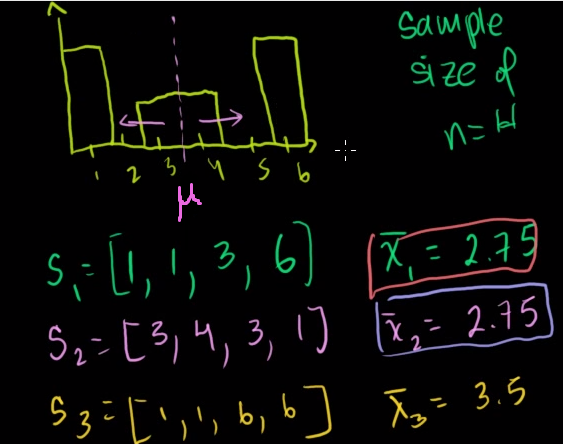
\includegraphics[scale=0.5]{img/Selection_005}
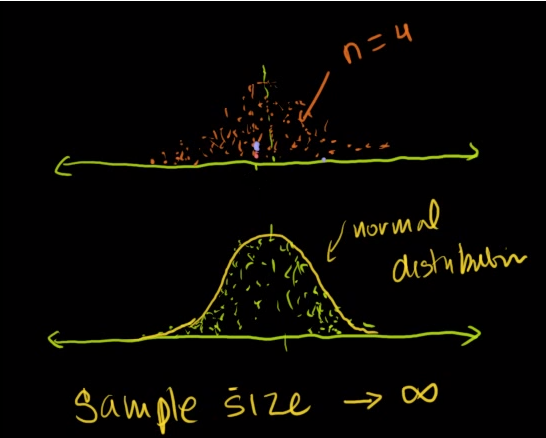
\includegraphics[scale=0.5]{img/Selection_006}
\end{figure}
Alt dette er kaldet for \textbf{fordeling af teststørrelsen}. Teststørrelsen fordeling har det samme gennemsnit, som den originale fordeling.
\begin{itemize}\itemsep-2pt
\item Der bliver taget $n$ stikprøver af sandsynlighedsfordelingen
\item Gennemsnittet af stikprøverne bliver plottet og danner en normalfordeling
\end{itemize}
En ideal normalfordeling har lige store arealer på højre-- og venstresiden af gennemsnittet, men hvis
\begin{itemize}\itemsep-2pt
\item der er mest på højresiden, så er den positiv skæv
\item der er mest på venstresiden, så er den negativ skæv
\end{itemize}
En ideal normalfordeling er ikke skæv.
\begin{figure}[H]
\centering
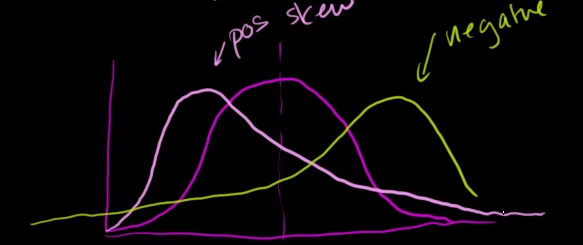
\includegraphics[scale=0.5]{img/Selection_007}
\end{figure}
\textbf{Kurtosis:} positiv kurtosis, så er der federe tail og mere spids peak. 
\begin{figure}[H]
\centering
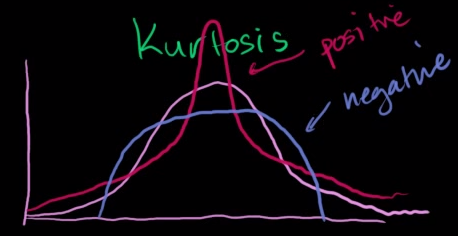
\includegraphics[scale=0.5]{img/Selection_008}
\end{figure}
Figuren nedenfor viser, hvordan man med større stikprøve størrelse, får en normalfordeling med en skævhed og kurtosis tættere på nul. 
\begin{figure}[H]
\centering
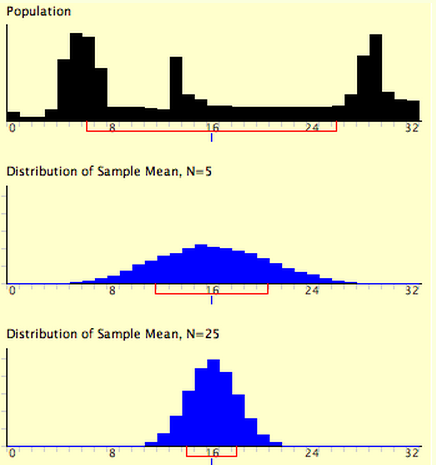
\includegraphics[scale=0.5]{img/Selection_009}
\end{figure}
\subsection{Standard Error for gennemsnittet}
Hvis man kender standard afvigelsen (eller variansen) og stikprøvestørrelsen, så kan standard afvigelsen for hver fordeling af teststørrelsen tilnærmelsesvis findes. Variansen for teststørrelse fordelingen er
$$\sigma^2_{\bar{x}}=\frac{\sigma^2}{n}$$
og standard afvigelsen er
$$\sigma_{\bar{x}}=\frac{\sigma}{\sqrt{n}}$$
Eksemplet nedenfor viser forskellige fordelinger af teststørrelser, og ud fra formlen kan det ses, at jo højere stikprøvestørrelsen er, jo lavere standard afvigelsen/varians vil man have i fordelingerne af teststørrelserne. 
\begin{figure}[H]
\centering
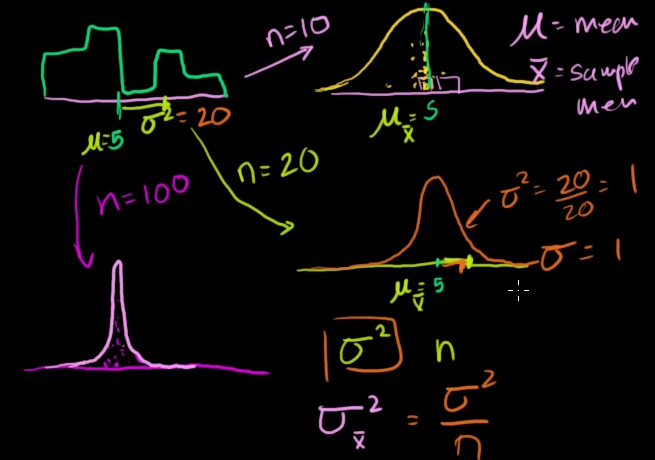
\includegraphics[scale=0.5]{img/Selection_010}
\end{figure}

\subsection{Eksempel på fordeling af teststørrelsen}
\begin{figure}[H]
\centering
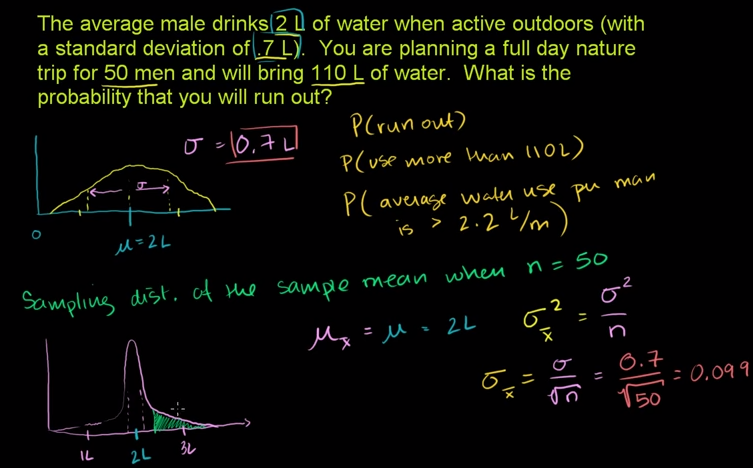
\includegraphics[scale=0.5]{img/Selection_013}
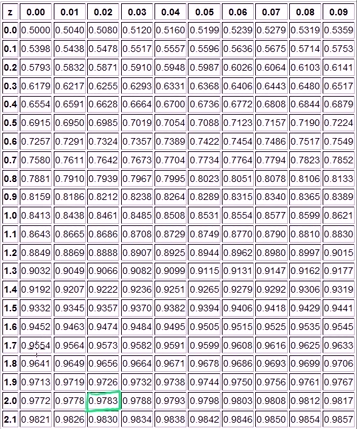
\includegraphics[scale=0.3]{img/Selection_012}
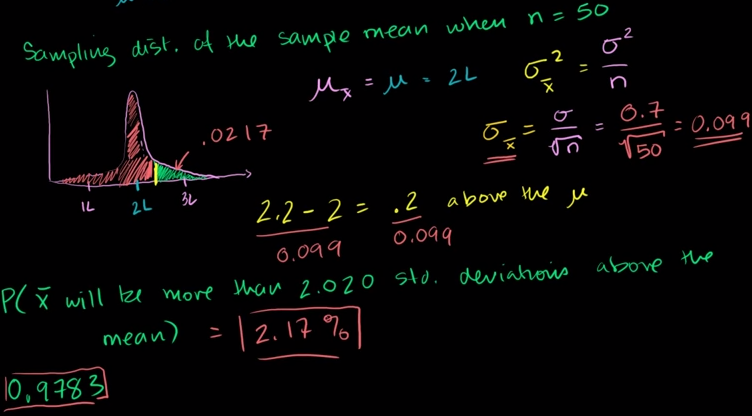
\includegraphics[scale=0.5]{img/Selection_011}
\end{figure}

\begin{figure}[H]
\centering
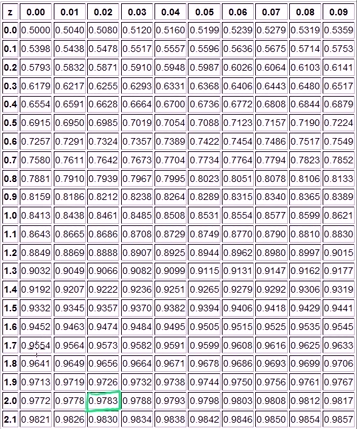
\includegraphics[scale=0.6]{img/Selection_012}
\end{figure}

% https://www.youtube.com/watch?v=0ZstEh_8bYc&list=PL1328115D3D8A2566&index=29


\subsection{Interval estimation (Confidence Intervals) (Ch.8)}
Den centrale grænseværdi; Hvis man fra en population med en vilkårlig fordeling tager stikprøver af størrelsen n, så vil gennemsnittene være tilnærmelsesvis normalfordelte. Jo større n er, jo nærmere kommer man en normalfordeling. Desuden vil variansen af denne normalfordeling falde, jo større n er,
$$Z=\frac{\bar{x}-\mu }{\sigma/\sqrt{n}}\sim N(0,1)$$
Hvis man tager stikprøver fra en standard normalfordeling N(0,1), ved man, at der
Eksempel: der bliver taget en stikprøve på 36 æbler fra en høst på over 200.000 æbler. Gennemsnitsvægten er stikprøven er 112 gram (med en standard afvigelsen på 40 gram). Hvad er sandsynligheden for at gennemsnitsvægten for alle æbler ligger enden for 100 og 124 gram?\\[0.2cm]
Vores population har en fordeling, med et gennemsnit, $\mu$, og en standard afvigelse, $\sigma$. Ud fra vores stikprøve vil vi få en fordeling af stikprøverne, der vil har det samme gennemsnit, $\mu_x$, og en standard afvigelse næsten lig med populationens standard afvigelse divideret med kvadratroden af vores antal stikprøver, således
$$\mu_{\bar{x}}=\mu$$
og 
$$\sigma_{\bar{x}}= \frac{\sigma}{\sqrt{n}}$$
hvor $n=36$. Men vi kender endnu ikke $\mu$.\\[0.2cm]
Der bliver spurgt om, hvad sandsynligheden er, at gennemsnitsvægten ligger inden for $\pm 12$ gram, således
$$P(\mu\text{ er indenfor 12 gram af vores }\bar{x})$$
Dette kan også skrives som
$$P(\bar{x}\text{ er indenfor 12 gram af vores }\mu)$$
Ved at formulere det sådan, så kan vores stikprøve fordeling bruges. Vi har et ukendt gennemsnit i stikprøve fordelingen, som er den sammen som populationens gennemsnit, og fordi de to er ens, så kan vi sige
$$P(\bar{x}\text{ er indenfor 12 gram af vores }\mu_{\bar{x}})$$
så hvis man kan finde ud af hvor mange standard afvigelser det er væk fra stikprøvens gennemsnit, $\mu_{\bar{x}}$, så kan z--tabellen bruges til at finde ud af hvad sandsynligheden er. Der er et problem, for vi ved ikke hvad den faktiske standard afvigelse for fordelingen er, vi ved kun at det er $$\sigma_{\bar{x}}= \frac{\sigma}{\sqrt{n}}$$
så vi laver en tilnærmelse af $\sigma$, for at løse problemet, således at vores standard afvigelse for stikprøverne er tilnærmelsesvis lig med populationens standard afvigelse
$$\sigma\approx s = 40\:gram$$
og nu kan vi regne sandsynligheden ud, ved først at regne standard afvigelsen ud
$$\sigma_{\bar{x}}=\frac{\sigma}{\sqrt{36}}=\frac{\sigma}{6}\approx \frac{s}{6}=\frac{40}{6}=6,67$$
så vores standard afvigelse for stikprøve fordelingen er 6,67 og for at finde sandsynligheden for at alle æblers vægt ligger mellem 100 og 124 gram, så divideres de 12 gram med 6,67, således
$$12/6,67=1,8$$
så på vores stikprøve fordeling er det 1,8 $\sigma_{\bar{x}}$ væk for gennemsnittet. Ved at kigge i z--tabellen, så kan vi finde værdien $0.9641$, men der skal trækkes 0.5 fra, for at få kun den ene halvdel med. Fordi det er en normal fordeling, så er den symetrisk omkring gennemsnittet, $\mu$, og vi kan gange den med to, for at få vores sandsynlighed, således
$$(0.9641-0.5)\cdot 2=0.9282$$
så der er 92.82\% chance for at den rent faktiske gennemsnit ligger indenfor 100 og 124 gram. 
\begin{figure}[H]
\centering
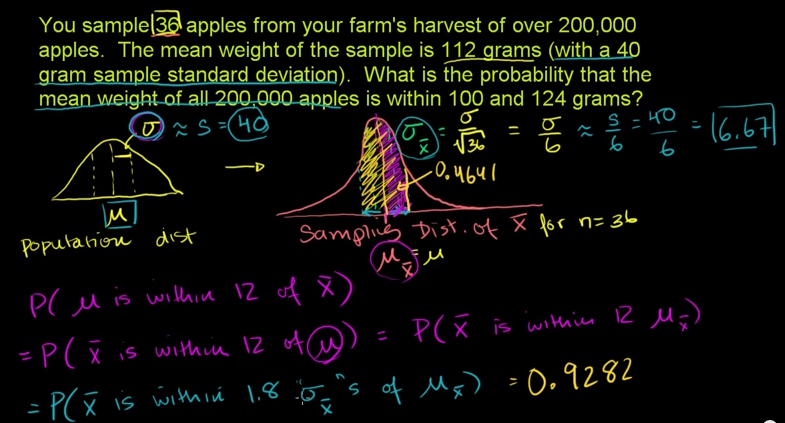
\includegraphics[scale=0.5]{img/Selection_004}
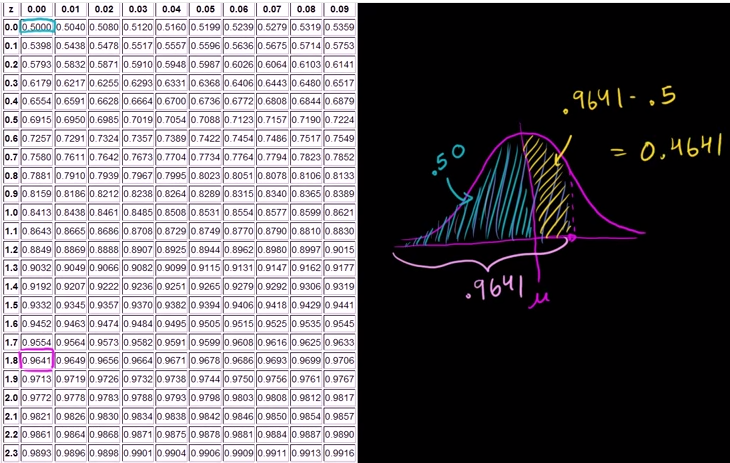
\includegraphics[scale=0.5]{img/Selection_003}
\end{figure}

\newpage
\section{Emne 3 -- Hypotesetestning}
\subsection{En population}
\subsubsection{En-- og tosidede hypotesetests}
Når man slår plat og krone, forventer man at få lige mange af hver. Man har altså en hypotese, som man ikke udtrykker klart, men som kan formuleres således: P(plat) = P(krone). Erfaring siger, at man ikke kan forvente præcis lige mange af hver. Der er en vis variation, og engang imellem kan man være meget uheldig, og andre gange kan man være meget heldig. Spørgsmålet er så, hvor uheldige man skal være, før man kan tillade sig at sætte spørgsmålstegn ved møntens ægthed. D.v.s, hvor skævt skal resultatet være, før man forkaster hypotesen og vælger en alternativ hypotese.\\[0.2cm]
Hvis man skal indføre en ny metode eller behandling, er man i reglen kun interesseret i, om den nye metode er bedre end den gamle. Hvis den nye er dårligere end den gamle, vil man selvfølgelig ikke have den, og hvis den kun er lige så god som den gamle, kan det nok ikke betale sig at indføre en ny metode. Man vil altså teste ensidigt:
\begin{eqnarray*}
H_0&:&\hspace{1cm}\text{Effekt af ny}=\text{Effekt af gammel}\\
H_1&:&\hspace{1cm}\text{Effekt af ny}>\text{Effekt af gammel}
\end{eqnarray*}
Hvis man derimod ønsker at teste f.eks. skoleformens indflydelse på rygning blandt skoleelever, kan man argumentere for, at skoleformerne kan virke begge veje, således at hypoteserne bør være:
\begin{eqnarray*}
H_0&:&\hspace{1cm}\text{Rygning blandt folkeskoleelever}=\text{Rygning blandt efterskoleelever}\\
H_1&:&\hspace{1cm}\text{Rygning blandt folkeskoleelever}>\text{Rygning blandt efterskoleelever}
\end{eqnarray*}
Den tosidede test giver en dobbelt så stor P-værdi som den ensidede test. P beregnes som sandsynligheden for at få noget, der er mere ekstremt end den fundne værdi. I den tosidige test er ekstreme værdier både større og mindre værdier. I den ensidige test ovenfor, er ekstreme værdier kun de store værdier for den ny effekt. Hvis man får en meget mindre effekt af den ny metode, skal man helt undlade at udføre testen. Hvis man gør det, vil man få en meget stor P-værdi.\\[0.2cm]
De mest enkle hypoteser sammenligner en eller anden parameter med et fast tal. Hvis man f.eks. laver lineær regression, tester man, om der er en stigende eller faldende sammenhæng mellem de to variable, og hypoteserne er:
\begin{eqnarray*}
H_0&:&\hspace{1cm}\text{Hældning}=0\\
H_1&:&\hspace{1cm}\text{Hældning}\neq 0
\end{eqnarray*}
Teststørrelsen er 
$$z_0=\frac{\bar{x}-\mu_0}{\sigma/\sqrt{n}}$$
Hvis P--værdien er under 0,05, så afvises $H_0$. 
\subsubsection{Type I og II fejl}
Når man laver en hypotesetest, kan man opskrive følgende tabel:
\begin{table}[H]
\centering
\begin{tabular}{|l|l|l|}
\hline
                     & $H_0$ er sand & $H_0$ er ikke sand \\ \hline
$H_0$ forkastes      & Type I fejl                           & OK                                         \\ \hline
$H_0$ forkastes ikke & OK                                    & Type II fejl                               \\ \hline
\end{tabular}
\end{table}
Når man tester en hypotese, vil der altid være en sandsynlighed for, at man forkaster hypotesen, selv om den er sand. Dette kaldes en Type I fejl, eller a i tabellen forneden. Sandsynligheden for en Type I fejl er den, man vælger som signifikantsniveau, altså a. Sandsynligheden for en Type II fejl kaldes b. Styrken defineres som 1--b, og er sandsynligheden for, at H0 forkastes, når den ikke er sand.
\begin{table}[H]
\centering
\begin{tabular}{|l|l|l|}
\hline
                     & $H_0$ er sand & $H_0$ er ikke sand \\ \hline
$H_0$ forkastes      & $\alpha$                           & $1-\beta$                                        \\ \hline
$H_0$ forkastes ikke & $1-\alpha$                                    & $\beta$                                        \\ \hline
\end{tabular}
\end{table}
\subsubsection{Tosidig hypotese om gennemsnittet}
Når man har en enkelt population, og ønsker at opstille en hypotese om middelværdien, skal man sammenligne middelværdien med en fast værdi, kaldet m0. Man kan skrive sin nulhypotese og alternative hypotese således:
\begin{eqnarray*}
H_0&:&\hspace{1cm}\mu =m_0\\
H_1&:&\hspace{1cm}\mu \neq m_0
\end{eqnarray*}
 	
\textbf{Konfidensintervaller omkring gennemsnittet:} Når man laver et tosidig t-test med signifikansniveau $\alpha$, kan man, i stedet for at se på P--værdien, se på det interval, hvor $H_0$ ikke forkastes. Ud fra t--værdien beregnes et 

\subsubsection{Ensidig hypotese om gennemsnittet}
Hvis man har en fast overbevisning om, at det, man undersøger, har et gennemsnit, der er enten større eller mindre end det faste tal, kan man lave en ensidig test.\begin{eqnarray*}
H_0&:&\hspace{1cm}\mu =m_0\\
H_1&:&\hspace{1cm}\mu < m_0
\end{eqnarray*}
eller
\begin{eqnarray*}
H_0&:&\hspace{1cm}\mu =m_0\\
H_1&:&\hspace{1cm}\mu > m_0
\end{eqnarray*}
Som eksempel, kunne det være at undersøge om der er mere fedt end angivet i en bestemt slags chips? Hypoteserne, der skal testes er nu
\begin{eqnarray*}
H_0&:&\hspace{1cm}\mu = 34g\\
H_1&:&\hspace{1cm}\mu > 34g
\end{eqnarray*}

\subsection{Eksempel med en population}
\subsection{Tosidede hypotesetests}
Først opstilles nul--hypotesen
$$H_0:\hspace{1cm}\text{Ingen effekt}$$
med andre ord, så vil gennemsnittet forblive det samme, dvs
$$\mu=1.2s$$
Den alternative hypotese er så
$$H_1:\hspace{1cm}\text{Har en effekt}$$
så det vil sige 
$$\mu\neq 1.2s$$
Først starter vi med at antage at $H_0$ er sandt, og ved at regne sandsynligheden for det, så kan det vurderes om det er sandt eller ej. Hvis sandsynligheden er lavere end 0.05, så antager man at det ikke er sandt.\\[0.2cm]
For at teste dette, så laver vi en stikprøve fordeling af det data vi har. Vi får så en normalfordeling og vi kan derfor antage at 
$$\mu_{\bar{x}}=\mu=1.2$$
Standard afvigelsen er så
$$\sigma_{\bar{x}}=\frac{\sigma}{\sqrt{n}}\approx\frac{s}{\sqrt{100}}=0.05$$
så 
$$\hat{\sigma_{\bar{x}}}=0.05$$
(Hat for at vise det er en approksimation)\\[0.2cm]
Så regnes teststørrelsen
$$z_0=\frac{\bar{x}-\mu_0}{\sigma/\sqrt{n}}=\frac{1.2-1.05}{0.05}=3$$
Så det er tre standard afvigelser væk fra gennemsnittet, $\mu$. Hvad er sandsynligheden så for at få et resultat der er længere væk fra gennemsnittet end tre standard afvigelser? (Både i den negative og positive retning)\\[0.2cm]
Ved at kigge i en z--tabel, så vil vi kunne se, at tre standard afvigelser ligger indenfor 99.7\% og derved er det kun 0.3\% der ligger udenfor, så sandsynligheden for at det ikke har nogen effekt er 0.003 og vi kan derfor afvise denne hypotese (fordi den er under 0.05).

\begin{figure}[H]
\centering
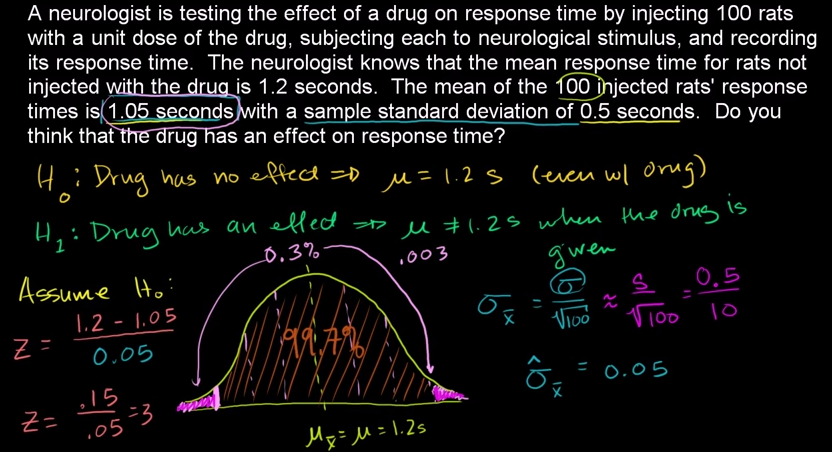
\includegraphics[scale=0.5]{img/Selection_014}
\end{figure}

% https://www.youtube.com/watch?v=-FtlH4svqx4&list=PL1328115D3D8A2566&index=37

\subsubsection{Ensidede hypotesetests}
Vi kan foretage en hypotesetest på den samme opgave, men nu fokuserer vi kun på den ene af enderne; enten er har den en positiv (sænker tiden) eller negativ effekt (øger tiden).\\[0.2cm] 
Vi har stadig den samme nul--hypotese
$$H_0:\hspace{1cm}\text{Ingen effekt}$$
med andre ord, så vil gennemsnittet forblive det samme, dvs
$$\mu=1.2s$$
Den alternative hypotese er så
$$H_1:\hspace{1cm}\text{Sænker responstiden}$$
så det vil sige 
$$\mu< 1.2s$$
Igen antager vi at $H_0$ er sand og kigger på hvad sandsynligheden er for $\mu=1.05s$. Så hvis $H_0$ er sandt, så
$$P(\text{Resultat lavere end 1.05s})=0.003/2=0.0015$$
Dette er meget usandsynligt, så vi afviser vores $H_0$ hypotese. 
\begin{figure}[H]
\centering
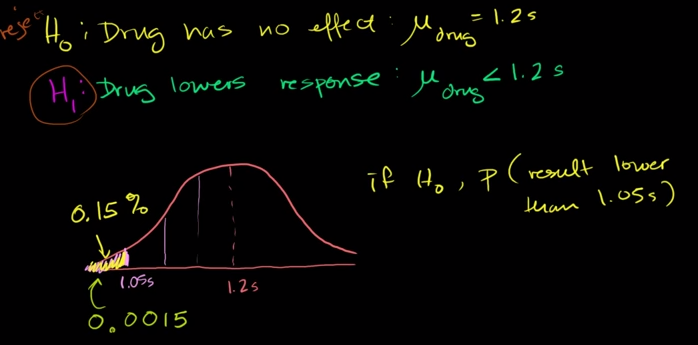
\includegraphics[scale=0.5]{img/Selection_015}
\end{figure}

% https://www.youtube.com/watch?v=mvye6X_0upA&index=38&list=PL1328115D3D8A2566

\subsection{To populationer}
Ofte har man flere grupper, som  man ønsker at sammenligne. Det simpleste tilfælde er at undersøge to ting af gangen.\\[0.2cm]
Der findes groft sagt to udgangspunkter: Enten ønsker man at sammenligne to naturligt forekommende grupper, eller også ønsker man at danne to grupper, som man så gør noget forskelligt ved. Disse grupper skal dannes så tilfældigt som muligt.\\[0.2cm]
For eksempel, I en undersøgelse af  brystkræftoperationer bliver patienterne fordelt tilfældigt i to grupper. Den ene gruppe får kun fjernet knuden, den anden gruppe får fjernet hele brystet. Patienterne er nødvendigvis vidende om behandlingens art, og resultatet kan være påvirket af patientens eget syn på behandlingen.\\[0.2cm]
I nogen tilfælde kan man danne grupper, hvor objekterne er parvis ens - eller endog samme objekt i to situationer.\\[0.2cm]
Når man skal sammenligne grupperne, kan man sammenligne gennemsnittene eller medianerne. For at sammenligne gennemsnittene, skal grupperne have ens varians. Men det kan være interessant i sig selv at undersøge om varianserne er ens.\\[0.2cm]
To sovemediciner giver begge en gennemsnitssøvn på 8 timer. Søvnen ved den ene varierer mellem 7 og 9 timer, søvnen ved den anden varierer mellem 2 og 18 timer. De fleste vil nok foretrække den første medicin.\\[0.2cm]
Hvis man har data fra to uafhængige populationer, kan man opstille hypoteserne
\begin{eqnarray*}
H_0&:&\hspace{1cm}\mu_1 = \mu_2\\
H_1&:&\hspace{1cm}\mu_1 \neq \mu_2
\end{eqnarray*}
eller
\begin{eqnarray*}
H_0&:&\hspace{1cm}\mu_1 = \mu_2\\
H_1&:&\hspace{1cm}\mu_1 < \mu_2
\end{eqnarray*}
eller
\begin{eqnarray*}
H_0&:&\hspace{1cm}\mu_1 = \mu_2\\
H_1&:&\hspace{1cm}\mu_1 > \mu_2
\end{eqnarray*}
Teststørrelsen er
$$z_0=\frac{\bar{x_1}-\bar{x_1}-\delta_0}{\sqrt{\frac{\sigma_1^2}{n_1}+\frac{\sigma_2^2}{n_2}}}$$
men vi er interesseret $\delta_0=0$, så
$$z_0=\frac{\bar{x_1}-\bar{x_1}-0}{\sqrt{\frac{\sigma_1^2}{n_1}+\frac{\sigma_2^2}{n_2}}}$$
For at fortsætte må man antage, at de to populationer er normalfordelte og har samme varians. (Det kræver en test. Denne varians skal estimeres. Det er ikke lovligt at tage det fælles estimat for de samlede data, da dette estimat anvender det fælles gennemsnit. Dette ville betyde, at man antager et fælles gennemsnit til at vise, om middelværdierne er ens. Man må i stedet beregne hver stikprøves varianser ud fra de faktiske gennemsnit. Man har:
$$\sigma^2_{\bar{X_1}-\bar{X_2}}=V(\bar{X_1}-\bar{X_2})=V(\bar{X_1})+V(\bar{X_2})=\frac{\sigma_1^2}{n_1}+\frac{\sigma_2^2}{n_2}=\frac{\sigma^2}{n_1}+\frac{\sigma^2}{n_2}$$
da vi antager at $\sigma^2_1=\sigma^2_2$

\subsubsection{Parvise tests}
For at lave t-testene i sidste afsnit antog man, at der var tale om to uafhængige populationer. Man kan også have eksempler, hvor populationerne ikke er uafhængige, idet observationerne i de to grupper er parrede. Der kan dreje sig om de samme patienter før og efter en behandling, eller individer, hvor man måler på højre og venstre hånd. Andre gange kan man stille forsøget således op, at man først går gennem den ret besværlige fase, hvor man parrer sine forsøgspersoner, så de er ens m.h.t. nogle relevante faktorer. Derefter fordeler man hvert par tilfældigt på de to behandlinger, som man ønsker at undersøge. Fordelen ved denne procedure er, at man fjerner en hel del af den variation, der naturligt er imellem forsøgspersoner.\\[0.2cm]
Beregningsmæssigt betyder dette, at man ser på forskellen mellem de to målinger indenfor hvert par, og i stedet for at regne med en varians i hver af de to grupper kan man nøjes med at se på variansen af denne forskel.\\[0.2cm]
Hvis man beregner forskellen mellem observationerne indenfor hvert par, kan man fortsætte beregningerne, som om man testede i en population.

\subsubsection{Hypoteser om varianser}
For at teste en hypotese af formen
\begin{eqnarray*}
H_0&:&\hspace{1cm}\sigma_1 = \sigma_2\\
H_1&:&\hspace{1cm}\sigma_1 \neq \sigma_2
\end{eqnarray*}
bruger man en varians ratio test. Man beregner en af disse to brøker:
$$F=\frac{s_1^2}{s_2^2}\hspace{1cm}eller\hspace{1cm}\frac{s_2^2}{s_1^2}$$
Teststørrelserne har en F-fordelingKapiletskift. Klik to gange for at komme tilbage med hhv. $(n_1,n_2)$ og $(n_2,n_1)$ frihedsgrader. Hvis man skal bruge tabelopslag, beregner man den af de to brøker, der giver $F>1$, og forkaster for $F > F_{tabelværdi}$.\\[0.2cm]
Hvis $P < 0,05$, forkastes H0. Varianserne er altså ikke ens. Hvis man fortsætter og tester for, om de har ens gennemsnit, forkaster man ikke - men resultatet er i bund og grund uinteressant.

\subsection{Z--statistik og T--statistik}
Hvis $s$ er lille ($n<30$ stikprøver), så skal der bruges samme fremgangsmåde til udregning af teststørrelsen, men i stedet for at bruge en z--tabel, så bruger man en t--tabel. 

\begin{figure}[H]
\centering
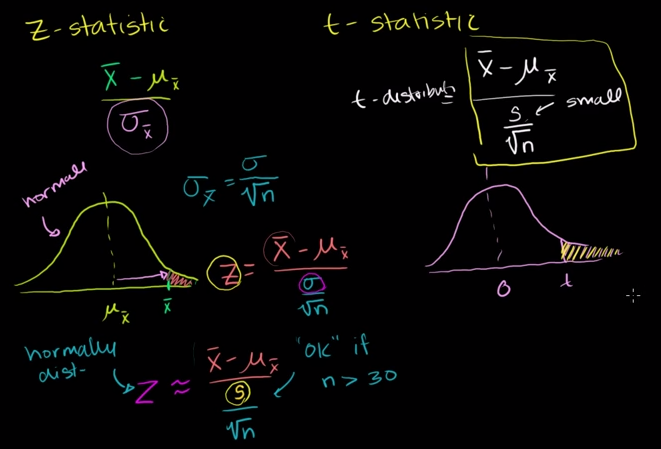
\includegraphics[scale=0.5]{img/Selection_016}
\end{figure}

% https://www.youtube.com/watch?v=5ABpqVSx33I&index=39&list=PL1328115D3D8A2566

\newpage
\section{Emne 4 -- Regression analyse}
\subsection{Simpel regression}
I alle de tidligere nævnte tests har man for hvert objekt kun målt 1 variabel. Derfor kaldes det også univariabel analyse. Hvis man måler flere ting, kaldes det multivariabel analyse.
Den simpleste model er lineær regression, hvor man har en uafhængig og en afhængig variabel, for eksempel vægt som funktion af højden.\\[0.2cm]
Formålet med regressionen er, at kunne forudsige noget om den afhængige variabel, hvis man kender den uafhængige. Der kan være andre variable, der også forudsiger noget om den afhængige variabel, og man kan derfor også lave modeller med flere uafhængige variable.\\[0.2cm]
Man kan også have variable, der varierer på en bestemt måde i forhold til hinanden, uden at der er tale om et direkte afhængighedsforhold. Der vil ofte være tale om en afhængighed af en helt tredie (fjerde, femte...) variabel. Der er så tale om korrelation.
\subsection{Den lineære model}
Den lineære regressionsligning er givet ved
$$Y=\beta_0+\beta_1x+\epsilon$$
hvor $\beta_0$ og $\beta_1$ er henholdsvis skæringen på y--aksen og hældningen. $\epsilon$ er den tilfældige afvigelse, da de enkelte observationspunkterne meget sjældent ligger lige på linien.\\[0.2cm]
Når man laver lineær regression skal man være meget opmærksom på observationer, der	ligger langt fra de andre, såkaldte ekstreme værdier. De kan have stor indflydelse på regressionsliniens hældning. Man bør undersøge om de skyldes en tastefejl, en  målefejl eller et objekt, der skal tages ud af undersøgelsen. Den røde figur viser en lineær regression og den blå figur er tilføjet en ekstreme værdi langt til højre for de andre punkter. Her er det tydeligt at se, hvad det har af betydning med de ekstreme værdier. 

\begin{figure}[H]
\centering
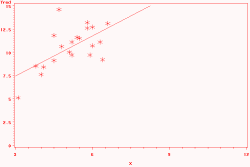
\includegraphics[scale=0.8]{img/regres1}
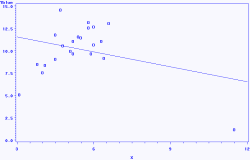
\includegraphics[scale=0.83]{img/regres3}
\end{figure}

\subsubsection{Estimation af $\beta_0$ og $\beta_1$}
Regressionslinen beregnes således, at man minimerer summen af kvadraterne på den lodrette afstand mellem punkterne og linien, og resultatet af minimeringen giver estimatet på $\beta_1$ som
$$\hat{\beta_1}=\frac{\sum^n_{i=1}y_i x_i-\frac{\left(\sum^n_{i=1}y_i\right)\left(\sum^n_{i=1}x_i\right)}{n}}{\sum^n_{i=1}x^2_i-\frac{\sum^n_{i=1}x_i}{n}}$$
og estimatet på $\beta_0$ får ved
$$\hat{\beta_0}=\bar{y}-\hat{\beta_1}\bar{x}$$
hvor $\bar{y}=(1/n)\sum^n_{i=1}y_i$ og $\bar{x}=(1/n)\sum^n_{i=1}x_i$.

\subsubsection{Sum af kvadrater i regression}
Den totale sum af kvadrater har $n - 1$ frihedsgrader og beregnes ved
$$SS_T=\sum^n_{i=1}(y_i-\bar{y})^2$$
Regressionens (modellens) afvigelse fra gennemsnittet har 1 frihedsgrad og beregnes ved
$$SS_M=\sum^n_{i=1}(\hat{y_i}-\bar{y})^2$$
Forskellen på $SS_T$ og $SS_M$ angiver, hvor meget punkterne varierer omkring den fundne linie. For hvert x kaldes afstanden mellem den observerede og den beregnede y-værdi for residualen. Den sidste sum af kvadrater kaldes derfor enten SSR eller SSE (for error). Her benyttes SSE ligesom i de tidligere variansanalyser.
$$SS_E=\sum^n_{i=1}e^2_i=\sum^n_{i=1}(y_i-\hat{y_i})^2$$
der har $n - 2$ frihedsgrader.\\[0.2cm]
Estimatet (unbiased) for variansen er
$$\sigma^2=\frac{SS_E}{n-2}$$

\subsubsection{Hypotesetest}
Hypoteserne i en lineær regression kan skrives
\begin{eqnarray*}
H_0&:&\hspace{1cm}\beta_1 = \beta_c\\
H_1&:&\hspace{1cm}\beta_1 \neq \beta_c
\end{eqnarray*}
hvor $\beta_c$ er den konstant vi ønsker at undersøge om hældningen er lig med. Man tester kun, om der er en stigende eller faldende sammenhæng mellem x og y. Man tester altså ikke, om denne sammenhæng er lineær.
\subsubsection{Konfidensintervaller}
\textbf{Konfidensinterval for hældnignen:} Til estimatet for $\beta_1$ kan man beregne et konfidensinterval. Man kan så tegne de to linier, hvis hældning er h.h.v. øverste og nederste konfidensgrænse for $\beta_1$. Det vil blive to linier, der roterer omkring punktet $\bar{y},\bar{x}$. Man vil se, at jo længere man bevæger sig væk fra fixpunktet, jo større er usikkerheden. Konfidensintervallet for hældningen $\beta_1$ er givet ved
$$\hat{\beta_1}-t_{\alpha/2,n-2}\sqrt{\frac{\hat{\sigma^2}}{S_{xx}}}\leq \beta_1\leq\hat{\beta_1}+t_{\alpha/2,n-2}\sqrt{\frac{\hat{\sigma^2}}{S_{xx}}}$$
\textbf{Konfidensinterval for det estimerede y:} $\beta_0$ er beregnet ud fra $\beta1$ og punktet $\bar{y},\bar{x}$. Da dette punkt også er et estimat, er der en usikkerhed herpå, og dermed er der en usikkerhed på $\beta_0$. Så man kan forestille sig, at konfidensgrænserne på den estimerede linie fås ved dels at vippe linien ligesom ovenfor og dels ved at skubbe linien lidt op og ned. Resultatet bliver et konfidensbånd omkring linien. Konfidensintervallet for 
 
\begin{figure}[H]
\centering
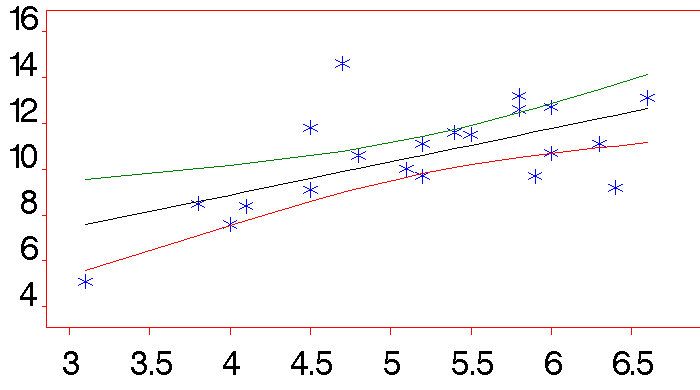
\includegraphics[scale=0.5]{img/Selection_017}
\end{figure}

\subsection{Korrelation}
Den lineære regression kræver, at den ene variabel kan siges at være afhængig af den anden. Hvis man derimod har to ligeværdige variable, der afhænger af hinanden, så må man nøjes med at lave en lineær korrelation. Korrelationskoefficienten beregnes som
$$R=\frac{\sum_{i=1}^nY_i(X_i-\bar{X})}{\left[\sum^n_{i=1}(X_i-\bar{X})^2\sum^n_{i=1}(Y_i-\bar{Y})^2\right]^{1/2}}$$
Hvis r er positiv, vil de to variable stige sammen, og det vil typisk vise sig ved, at punkterne ligger i en sværm, der ligger på skrå opad til højre, mens en negativ korrelation betyder, at den ene variabel stiger, når den anden falder, så sværmen af punkter går nedad mod højre. Der er dog ingen garanti for, at punkterne ligger på linie, se næste afsnit.\\[0.2cm]
Der er to meget udbredte misforståelser om r (eller r2). Selv om eksemplerne her formuleres om lineær regression, gælder det samme i korrelationsanalyse, hvor man godt nok ikke må lave en ret linie, men hvor man alligevel har en ide om fordelingen at data.
\begin{enumerate}\itemsep-2pt
\item Korrelationskoefficienten måler ikke størrelsen af liniens hældning
\begin{figure}[H]
\centering
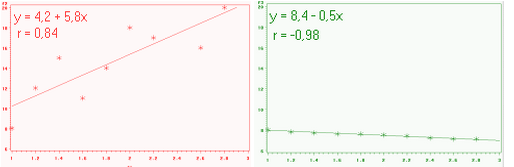
\includegraphics[scale=0.5]{img/Selection_018}
\end{figure}
\item Korrelationskoefficienten måler ikke, hvor godt en ret linie passer
\begin{figure}[H]
\centering
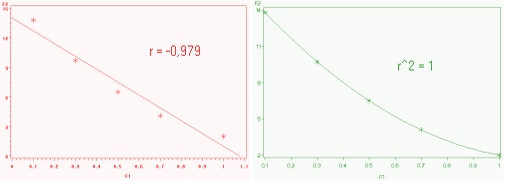
\includegraphics[scale=0.5]{img/Selection_019}
\end{figure}
\end{enumerate}

\subsection{Eksempel}
\subsubsection{Squared Error}
Tegn en masse punkter i koordinatsystemet og en linje der har den mindste fejl (den vertikale afstand op til regressions linjen)
\begin{figure}[H]
\centering
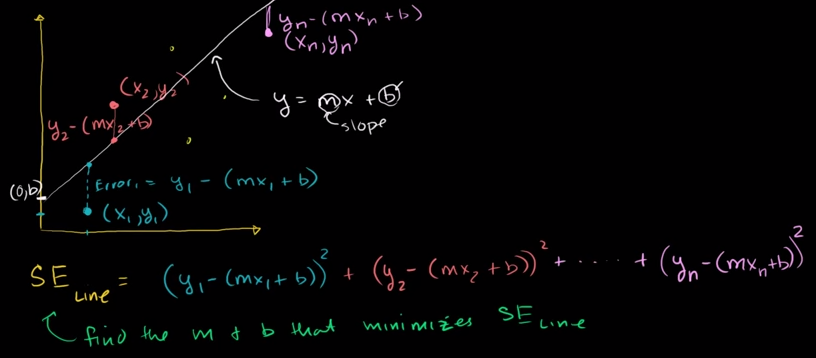
\includegraphics[scale=0.5]{img/Selection_020}
\end{figure}
Prøv med tre punkter; $\hspace{1cm}(1,2)\hspace{1cm}(2,1)\hspace{1cm}(4,3)$\\[0.2cm]
Find så
\begin{itemize}\itemsep-2pt
\item Gennemsnittet af x'erne
$$\bar{x}=\frac{1+2+4}{3}=7/3$$
\item Gennemsnittet af y'erne
$$\bar{y}=\frac{2+1+3}{3}=2$$
\item Gennemsnittet af punkterne
$$\bar{xy}=\frac{1\cdot 2+2\cdot 1+4\cdot 3}{3}=16/3$$
\item Gennemsnittet af de kvadrede x'er
$$\bar{x^2}=\frac{1^2+2^2+4^2}{3}=21/3=7$$
\end{itemize}
Med udregning, så får vi en hældning på
$$\beta_1=3/7$$
og vi kan nu finde skæringen på y--aksen, således
$$\beta_0=2-\frac{3}{7}\cdot \frac{7}{3}=1$$
Så det færdige udtryk for vores regressions linje er
$$y=\frac{3}{7}x+1$$
\begin{figure}[H]
\centering
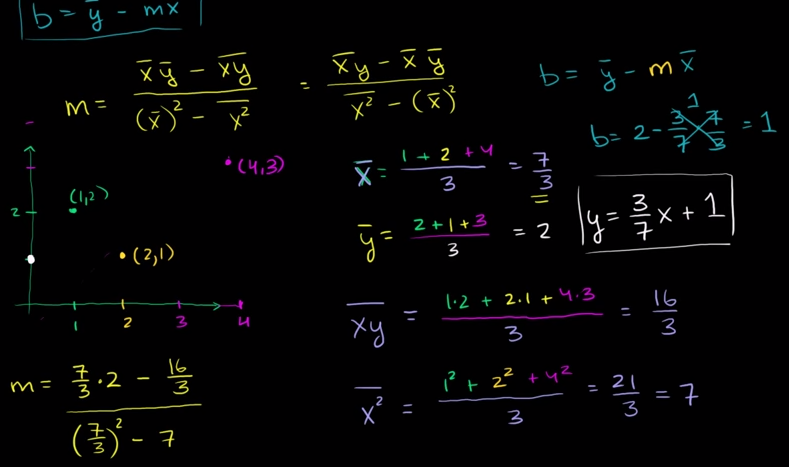
\includegraphics[scale=0.5]{img/Selection_021}
\end{figure}

\subsubsection{R--Squared (Coefficient of Determination)}
Efter at have fundet regressions ligningen, så kan det være en fordel at kigge på, hvor godt linjen passer på datasættet. 
$$SE_{line}=(y_1-(\beta_0+\beta_1x_1))^2+(y_2-(\beta_0+\beta_1x_2))^2+\cdots+(y_n-(\beta_0+\beta_1x_n))^2$$
Med andre ord, hvor meget (procent) af den totale variation i y er beskrevet af variationen i x?\\[0.2cm]
Den totale variation i y (Squared Error of $\bar{y}$) er givet ved
$$SE_{\bar{y}}(y_1-\bar{y})^2+(y_2-\bar{y})^2+\cdots+(y_n-\bar{y})^2$$
Hvor meget af den totale variation er \textbf{ikke} beskrevet af regressions linjen? 
$$\frac{SE_{line}}{SE_{\bar{y}}}$$
så for at finde $r^2$
$$r^2=1-\frac{SE_{line}}{SE_{\bar{y}}}$$
hvis $SE_{line}$ er er lavt, så er det et godt fit, og derfor tæt på 1. 


\subsection{Andre regression}
Den polynomielle regression af grad $n$ er givet ved ligningen
$$Y=\beta_0+\beta_1x_1+\beta_2x_2^2+\cdots+\beta_i+x_i^n+\epsilon$$
Hvor $\epsilon$ er fejlen, og summen af $\epsilon$'erne er lig nul.

Den multipel regression med $k$ regressions variable er givet ved
$$Y=\beta_0+\beta_1x_1+\beta_2x_2+\cdots+\beta_k+x_k+\epsilon$$
Hvor $\epsilon$ er fejlen, og summen af $\epsilon$'erne er lig nul. De uafhængige variable skal være indbyrdes uafhængige og ukorrelerede.\\[0.2cm]
Estimatet (unbiased) af variansen for en multipel regression er
$$\hat{\sigma^2}=\frac{\sum^n_{i=1}e^2_i}{n-p}=\frac{SS_E}{n-p}$$
Den overordnede hypotese er
\begin{eqnarray*}
H_0&:&\hspace{1cm}\beta_1 = \beta_2 = \cdots =\beta_k = 0\\
H_1&:&\hspace{1cm}\beta_j \neq 0\text{, for mindst et }j
\end{eqnarray*}


\newpage
\section{Emne 5 -- Analyse af variance}
\subsection{Analysis Of Variance -- Envejs (ANOVA 1 (Ch.13))}
Hvis man har flere end to populationer, er det ikke praktisk at sammenligne dem to og to, da det giver en meget stor Type I fejl. Selv om man bruger en $\alpha$ på 0,05 hver gang, vil den samlede Type I fejl blive meget større. Hvis der er 4 populationer, er der 6 sammenligninger, og sandsynligheden for ikke at forkaste nogen af de 6, hvis $H_0$ er sand, er 0,95 = 0,74. Derved bliver sandsynligheden for mindst 1 Type I fejl = 1 - 0,95 = 0,26. I stedet bør man bruge en test, hvor den samlede sandsynlighed for Type I fejl er det valgte a.\\[0.2cm]
\textbf{ANOVA 1:} I første omgang nøjes man med at teste den noget simple hypotese
\begin{eqnarray*}
H_0&:&\hspace{1cm}\tau_1 = \tau_2 = \cdots =\tau_k\\
H_1&:&\hspace{1cm}\text{Ikke alle $tau$'erne er ens}
\end{eqnarray*}
Man tester hypotesen ved at se på forskellige former for variation. Derfor har testen fået navnet Analysis Of Variance.\\[0.2cm]
I stedet for at sige, at man har forskellige grupper, kan man sige, at man har en faktor med forskellige niveauer (deraf navnet envejs variansanalyse). Den variabel, der angiver disse niveauer, kaldes den uafhængige variabel. De målinger, man foretager, afhænger af hvilket niveau, man er på, og de kaldes derfor den afhængige variabel.
\subsubsection{Antagelser}
Når man laver en variansanalyse, antager man, at observationerne kommer fra uafhængige, normalfordelte populationer med ens varians. Testen er meget pålidelig selv ved store afvigelser fra normalfordelingen, bare stikprøverne ikke er for små. Ligeledes kan testen tåle store afvigelser indenfor varianserne, bare stikprøvestørrelserne fra de forskellige populationer er ens eller næsten ens.\\[0.2cm]
Hvis man kigger nærmere på t-testen i to populationer, vil man se, at man i brøken sammenligner afstanden mellem de to gennemsnit (i tælleren) med spredningen (i nævneren). Man får en numerisk stor t-værdi, når afstanden mellem gennemsnittene er stor i forhold til spredningen, og en stor t-værdi betyder, at man forkaster hypotesen om ens gennemsnit.\\[0.2cm]
Når man vil teste hypotesen $H_0$ mod $H_1$, så sammenligner man variationen indenfor grupperne med variationen mellem grupperne. Hvis variationen indenfor grupperne er lille i forhold til variationen mellem grupperne, forkaster man hypotesen om ens gennemsnit.
\begin{figure}[H]
\centering
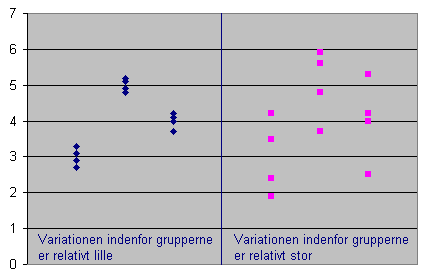
\includegraphics[scale=0.5]{img/Selection_022}
\end{figure}
Det ser umiddelbart ud til, at der er forskel på de tre grupper til venstre, mens der måske ikke er signifikant forskel på grupperne til højre. 
\subsubsection{Modellen}
Envejs variansanalyse og t-test anvendes til eksperimenter med et meget simpelt design: 1 - 2 - mange grupper, der kun skal testes for forskellighed. Eksperimenter kan laves med meget mere indviklet design, og man kan teste for mange andre sammenhænge end blot forskellighed (tænk bare på lineær regression). Derfor er der brug for at beskrive design og sammenhænge med en matematisk model. Den model, der kan opskrive for både envejs variansanalyse og t-test, er
$$Y_{ij}=\mu_i+\epsilon_{ij}$$
hvor $Y_{ij}$ er den j'te observation i det i'te niveau af faktoren i den i'te gruppe, $\mu_i=\mu+\tau_i$ er gennemsnittet af det i'te observation og $\epsilon_{ij}$ er en eksperimentel fejl.
\subsubsection{Summer af kvadrater (Sums of Squares -- $SS_T$)}
Størrelsen $SS_E$, der er variationen indenfor grupperne, kaldes også error sums of squares eller residual sums of squares, $SS_R$. Ud fra modellen beregnes her variationen på den normalfordelte eksperimentelle fejl
$$SS_E=\text{Indenfor grupperne SS}=\sum^k_{i=1}\sum^{n_i}_{j=1} (y_{ij}-\hat{y_{i\bullet}})^2 $$
med frihedsgraderne 
$$a(n-1)$$
Variationen mellem grupperne (gruppe sums of squares) er i modellen forklaret vha. a'erne. Da denne ene faktor kan kaldes A, benævnes variationen $SS_A$. Den beregnes ved
$$SS_A=\text{Mellem gurpperne SS}=\sum^k_{i=1}n_i(\bar{y_{i\bullet}}-\bar{y_{\bullet\bullet}})^2$$
med frihedsgraderne
$$a-1$$
Til sidst er der den totale variation, der også er summen af de to andre
$$SS_T=SS_E+SS_A=\sum$$
med frihedsgraderne
$$an-1$$
Estimatet indenfor grupperne er givet ved
$$MS_E=\text{Error mean square}=\frac{SS_E}{(a(n-1))}$$
Fra SSA beregner man mellem-gruppe-variansen, der altså sammenligner gruppernes gennemsnit med det fælles gennemsnit, således
$$MS_A=\frac{SS_A}{a-1}$$
Under $H_0$ er $MS_A$ også et estimat på $s^2$, da
$$\sum^a_{i=1}\tau_i=0$$
Teststørrelsen bliver herefter
$$F_0=\frac{MS_A}{MS_E}$$
Hvis $H_0$ er sand, burde F være tæt på 1, da $MS_E$ og $MS_A$ estimerer samme størrelse. Hvis $MS_A$ derimod er stor i forhold til $MS_E$, kan det skyldes, at $tau$'erne ikke er 0, og derved bliver F stor, og så forkastes hypotesen om ens middelværdi. Hvis $H_1$ er sand, så $MS_A$ et estimat på $s^2$ plus et positiv udtryk der inkorporerer variation som følge af systematisk forskel i gennemsnittene.

\subsubsection{ANOVA test}
Testen skrives op på følgende måde:
\begin{table}[H]
\centering
\begin{tabular}{lllll}
Source of Variation & Sums of Squares & Degrees of Freedom & Mean Square & $F_0$               \\
Model               & $SS_A$          & a-1                & $MS_A$      & $\frac{MS_A}{MS_E}$ \\
Error               & $SS_E$          & $a(n-1)$           & $MS_E$      &                     \\
Total               & $SS_T$          & $an-1$             &             &                    
\end{tabular}
\end{table}
Hvis $k = 2$ giver ANOVA testen samme resultat som t-testen, idet teststørrelserne opfylder at $F = t^2$, og fordelingerne opfylder at $F(1,N - 2) = t(N - 2)^2$.\\[0.2cm]
\textbf{To typer ANOVA:} Man skelner mellem to typer eksperimenter
\begin{itemize}\itemsep-2pt
\item I "fast faktor" modellen er de forskellige grupper faste, d.v.s. de er valgt, fordi netop de grupper har interesse. Det kan være nogle bestemte typer af behandling, som man vil sammenligne, og konklusionen af testen vil kun omhandle de anvendte behandlinger.
\item I "tilfældig faktor" modellen er de forskellige grupper valgt tilfældigt ud fra en større mængde af mulige emner. Det kan f.eks. være 4 sygehuse i mindre danske byer. Man ønsker at drage en konklusion om den større gruppe, så hypotesen bør formuleres "Der er ikke forskel på ..... i sygehusene i mindre danske byer".
\end{itemize} 
Så længe man kun har 1 faktor (1 gruppeinddeling), udføres ANOVA testen nøjagtig ens i de to modeller.

\subsection{Analysis Of Variance -- Tovejs (ANOVA 2 (Ch.14))}
Envejs variansanalyse (ANOVA 1) blev introduceret som en udvidelse af t--testen til at analysere flere end to grupper. Disse grupper må nødvendigvis have et overordnet faktor. De enkelte grupper kaldes så niveauer af denne faktor. Et eksempel kunne være 
\begin{table}[H]
\centering
\begin{tabular}{ll}
\textbf{Faktor} & \textbf{Niveauer}                                               \\
Køn             & Mand, kvinde                                                    \\
Diæt            & Kontrol(anbefalet energifordeling), høj fedt\%, høj kulhydrat\%
\end{tabular}
\end{table}
Hvis nu man undersøger vægtændring (den afhængige variabel) og ser på effekten af de forskellig diæter, så kunne det jo være interessant at se, om effekten er den samme hos mænd og kvinder. Derfor vil man gerne se på de to faktorer samtidig, og man får brug for tovejs variansanalyse. Man kunne tilføje en tredie faktor, f.eks. aldersgruppe, og så bruge trevejs variansanalyse. Her skal kun gennemgås tovejs variansanalyse.

\subsubsection{Antagelser}
Når man laver en variansanalyse, antager man, at observationerne kommer fra uafhængige, normalfordelte populationer med ens varians. Testen er meget pålidelig selv ved store afvigelser fra normalfordelingen, bare stikprøverne ikke er for små. Ligeledes kan testen tåle store afvigelser indenfor varianserne, bare stikprøvestørrelserne fra de forskellige populationer er ens eller næsten ens.\\[0.2cm]
\textbf{Balanceret krydsdesign:} Hvis hvert niveau af den ene faktor optræder i kombination med hvert niveau af den anden faktor, sige man, at de to faktorer er krydsede. Man stiller sine data op i en tabel, hvor den ene faktor er repræsenteret i søjlerne og den anden faktor er repræsenteret af rækkerne. Hver niveau kombination kaldes en celle. Antallet af observationer i den i'te række og j'te celle kaldes $n_{ij}$. Hvis der er lige mange observationer i hver celle, har man et balanceret design.
\begin{table}[H]
\centering
\begin{tabular}{llll}
\textbf{Køn \textbackslash Diæt} & Normal        & Fedtrig       & Kulhydratrig  \\
Mænd                             & $n_{11}=n$ = n; `x11 & n12 = n; `x12 & n13 = n; `x13 \\
Kvinder                          & n21 = n; `x11 & n22 = n; `x11 & n23 = n; `x11
\end{tabular}
\end{table}
Den afhængige variabel er vægtændring.\\[0.2cm]
Der kan opstille tre nul--hypoteser
\begin{eqnarray*}
H_0&:&\hspace{1cm}\text{Der er ingen interaktion mellem køn og diæt}\\
H_0&:&\hspace{1cm}\text{Køn har ingen effekt på vægtændringen}\\
H_0&:&\hspace{1cm}\text{Diæt har ingen effekt på vægtændringen}
\end{eqnarray*}
Hypotesen om interaktion er med vilje sat øverst, selv om den i tabellerne står nederst. Man bør nemlig først teste for interaktionen. Hvis H0 ikke forkastes, d.v.s. at der ikke er interaktion, så går man videre og tester, om der er nogen effekt af de to faktorer. Hvis man til gengæld forkaster og altså finder en interaktion, så anbefales det, at man stopper der og ikke tester, om der er en effekt af de enkelte faktorer (kaldet main effekt eller hovedeffekten), da disse tests så ikke er gyldige (se eksempel 5 i næste afsnit). Der kan dog være situationer, hvor man ønsker at teste for hovedeffekterne, men man må så gøre sig selv og andre klart, hvordan hovedeffekterne skal forstås i netop denne situation.\\[0.2cm]
For at lave en skitse af effekterne afsætter man cellernes gennemsnit i et koordinatsystem, hvor niveauerne af den ene faktor er afsat på x--aksen. For hvert niveau af den anden faktor, forbinder man de tilhørende gennemsnit. Man behøver kun at lave én figur. Nedenfor er begge mulige skitser med for at fremme forståelsen. Der er vist forskellige scenarier, når faktor A har niveauerne P1 og P2, mens faktor B har niveauerne 1, 2 og 3, og man har målt en point scoring
\begin{figure}[H]
\centering
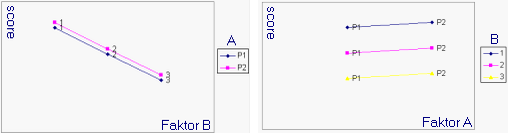
\includegraphics[scale=0.5]{img/Selection_023}
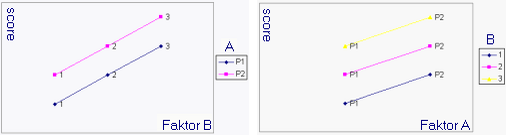
\includegraphics[scale=0.5]{img/Selection_024}
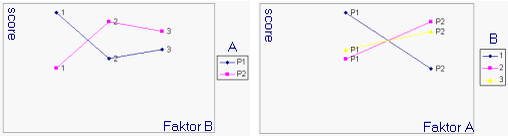
\includegraphics[scale=0.5]{img/Selection_025}
\end{figure}
Når der ikke er interaktion, er linierne nogenlunde parallelle, og en eventuel effekt af faktorerne viser sig ved, at linierne parallelforskydes væk fra hinanden. Man skal selvfølgelig teste for at se, om effekterne er signifikante. Interaktion viser sig ved, at linierne ikke er parallelle - men man skal selvfølgelig teste, om denne interaktion er signifikant. Hvordan skal interaktionen så forstås?\\[0.2cm]
Antag, at man måler muskelstyrke hos unge og gamle, hvoraf nogle er raske og andre har en sygdom, der svækker musklerne.
\begin{figure}[H]
\centering
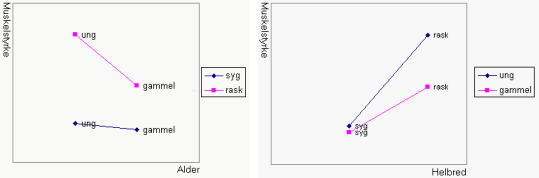
\includegraphics[scale=0.5]{img/Selection_026}
\end{figure}
På figurerne ses klart en interaktion. På venstre figur er der en tydelig effekt af alder hos de raske, hvorimod der næsten ingen effekt er af alder hos de syge. Ser man i stedet på højre figur, kan man se, at der er en effekt af sygdommen,\textit{ men denne effekt er ikke lige stor hos unge og gamle.} Hvis testen viser, at denne interaktion er signifikant, så er der jo ingen grund til at teste for en separat effekt af alder eller af sygdom, for disse effekt er jo netop indbygget i interaktionen, jvf. det, der er skrevet med kursiv.

\subsubsection{Modellen}
Modellen for det balancerede krydsdesign er
$$Y_{ijk}=\mu+\tau_i+\beta_j+(\tau\beta)_{ij}+\epsilon_{ijk}$$
hvor $Y_{ijk}$ er den k'te observation på det i'te niveau af faktor A og det j'te niveau af faktor B, $\mu$ er gennemsnittet af det hele, $\tau_i$ er effekten af niveau i af faktor A, $\beta_j$ er effekten af niveau j af faktor B, $(\tau\beta)_{ij}$ er interaktionen mellem niveau i af faktor A med niveau j af faktor B og $\epsilon_{ijk}$ er en normalfordelt eksperimentel fejl.\\[0.2cm]
Hypoteserne kan skrives som
\begin{eqnarray*}
H_0&:&\hspace{1cm}\tau_1=\tau_2=\cdots=\tau_a=0\hspace{0.5cm}\text{Ingen main effekt for faktor A}\\
H_1&:&\hspace{1cm}\text{Mindste en }\tau_i\neq 0\\
H_0&:&\hspace{1cm}\beta_1=\beta_2=\cdots=\beta_b=0\hspace{0.5cm}\text{Ingen main effekt for faktor B}\\
H_1&:&\hspace{1cm}\text{Mindste en }\beta_j\neq 0\\
H_0&:&\hspace{1cm}(\tau\beta)_{11}=(\tau\beta)_{12}=\cdots=(\tau\beta)_{ab}=0\hspace{0.5cm}\text{Ingen interaktion}\\
H_1&:&\hspace{1cm}\text{Mindste en }(\tau\beta)_{ij}\neq 0
\end{eqnarray*}

\subsubsection{Summer af kvadrater}
Den totale variation fås ved formlen
$$SS_T=\sum_{i=1}^a\sum_{j=1}^b\sum_{k=1}^n(y_{ijk}-\bar{y_{\bullet\bullet\bullet}})^2$$
med frihedsgraderne $a-1$.\\[0.2cm]
Som i envejs ANOVA kan $SS_T$ deles i to portioner, $SS_E$, der er variationen indenfor grupperne og $SS_M$, der er variationen mellem grupperne og derfor den variation, der skal beskrives ved modellen
$$SS_E=\sum_{i=1}^a\sum_{j=1}^b\sum_{k=1}^n(y_{ijk}-\bar{y_{ij\bullet}})^2$$
med frihedsgrader $ab(n-1)$.
$$SS_M=\sum_{i=1}^a\sum_{j=1}^b\sum_{k=1}^n(\bar{y_{ij\bullet}}-\bar{y_{i\bullet\bullet}}-\bar{y_{\bullet j\bullet}}-\bar{y_{\bullet\bullet\bullet}})^2$$
med frihedsgrader $ab-1$.\\[0.2cm]
For at lave tovejs ANOVA skal man dele variationen mellem celler op i tre komponenter: et bidrag fra faktor A, et bidrag fra faktor B og endelig et bidrag fra interaktionen.\\[0.2cm]
Variationen mellem niveauerne af faktor A beregnes ved
$$SS_A=an\sum_{i=1}^a\sum_{j=1}^b\sum_{k=1}^n(y_{\bullet j\bullet}-\bar{y_{\bullet\bullet\bullet}})^2$$
med frihedsgraden $a-1$. \\[0.2cm]
Tilsvarende fås variationen mellem niveauerne af faktor B ved
$$SS_B=\sum_{i=1}^a\sum_{j=1}^b\sum_{k=1}^n(y_{i\bullet\bullet}-\bar{y_{\bullet\bullet\bullet}})^2$$
med frihedsgraden $b-1$. \\[0.2cm]
Endelig fås variationen fra interaktionen ved
$SS_I=SS_M-SS_A-SS_B$
med frihedsgraden $(a-1)(b-1)$. \\[0.2cm]
Alt i alt får man så at
$$SS_T=SS_A+SS_B+SS_I+SS_E$$
med frihedsgraden $abn-1$. \\[0.2cm]
Teststørrelsen for
\begin{itemize}\itemsep-2pt
\item Faktor A
$$F_0=\frac{MS_A}{MS_E}$$
\item Faktor B
$$\frac{MS_B}{MS_E}$$
\item Interaktion mellem A og B
$$\frac{MS_{I}}{MS_E}$$
\end{itemize}
hvor 
$$MS_A=\frac{SS_A}{a-1}$$
$$MS_B=\frac{SS_B}{b-1}$$
$$MS_I=\frac{SS_I}{(a-1)(b-1)}$$
$$MS_E=\frac{SS_E}{ab(n-1)}$$

\begin{table}[H]
\centering
\begin{tabular}{lllll}
Source of Variation & Sums of Squares & Degrees of Freedom & Mean Square & $F_0$               \\
Faktor A               & $SS_A$          & a-1                & $MS_A=\frac{SS_A}{a-1}$      & $\frac{MS_A}{MS_E}$ \\
Faktor B               & $SS_B$          & b-1                & $MS_B=\frac{SS_B}{b-1}$      & $\frac{MS_B}{MS_E}$ \\
Interaktion              & $SS_I$          & (a-1)(b-1)                & $MS_I=\frac{SS_I}{(a-1)(b-1)}$      & $\frac{MS_I}{MS_E}$ \\
Error               & $SS_E$          & $ab(n-1)$           & $MS_E=\frac{SS_E}{ab(n-1)}$      &                     \\
Total               & $SS_T$          & $abn-1$             &             &                    
\end{tabular}
\end{table}

\newpage
\subsection{Eksempel}
Datasæt; tre forskellige slags lægemiddel til en gruppe mennesker
\begin{eqnarray*}
1&:&\hspace{0.5cm}3\hspace{0.2cm}2\hspace{0.2cm}1\\
2&:&\hspace{0.5cm}5\hspace{0.2cm}3\hspace{0.2cm}4\\
3&:&\hspace{0.5cm}5\hspace{0.2cm}6\hspace{0.2cm}7
\end{eqnarray*}
Det samlede gennemsnit
$$\bar{x}=\frac{3+2+1+5+3+4+5+6+7}{9}=4$$
giver det samme som at tage de enkeltes gennemsnit og så gennemsnittet af det
\begin{eqnarray*}
\bar{x_1}&:&\hspace{0.5cm} \frac{3+2+1}{3}=2\\
\bar{x_2}&:&\hspace{0.5cm} \frac{5+3+4}{3}=4\\
\bar{x_3}&:&\hspace{0.5cm} \frac{5+6+7}{3}=6
\end{eqnarray*}
Total sum of Squares
$$SS_T=(3-4)^2+(2-4)^2+(1-4)^2+(5-4)^2+(3-4)^2+(4-4)^2+(5-4)^2+(6-4)^2+(7-4)^2=30$$
SS indenfor grupperne er givet ved
$$SS_E=(3-2)^2+(2-2)^2+(1-2)^2+(5-4)^2+(3-4)^2+(4-4)^2+(5-6)^2+(6-6)^2+(7-6)^2=6$$
I stedet for at tage afstanden fra det samlede gennemsnit, så tages der nu afstand for hver gruppes gennemsnit, for at finde hvor stor variationen er.\\[0.2cm] 
SS mellem gurpperne er givet ved
$$SS_A=3\cdot(2+4)^2+3\cdot(4+4)^2+3\cdot(6+4)^2=24$$
hvilket også giver god mening, for 
$$SS_T=SS_E+SS_A$$
Hypoteser
\begin{eqnarray*}
H_0&:&\hspace{0.5cm}\text{Lægemidlerne har ikke nogen effekt}\hspace{0.5cm}\mu_1=\mu_2=\mu_3\\
H_1&:&\hspace{0.5cm}\text{Lægemidlerne har en effekt}
\end{eqnarray*}
Gå ud fra at $H_0$ er sand og udregn teststørrelsen
$$F_0=\frac{MS_A}{MS_E}=\frac{12}{1}=12$$
Rimeligt højt tal. Aflæs i F--tabel med en $\alpha=0.10$ og med DoF 2 og 6, så finder vi en 
$$F_c=3,46$$
og vi kan så afvise $H_0$ fordi vores teststørrelse er langt større en vores critical F. 







































\end{document}